% !TEX spellcheck = en_US
% !TEX spellcheck = LaTeX

\documentclass[letterpaper,english,10pt]{article}


\usepackage{%
	amsfonts,%
	amsmath,%	
	amssymb,%
	amsthm,%
	babel,%
	bbm,%
	%biblatex,%
	caption,%
	centernot,%
	color,%
	enumerate,%
	%enumitem,%
	epsfig,%
	epstopdf,%
	etex,%
	fancybox,%
	framed,%
	fullpage,%
	%geometry,%
	graphicx,%
	hyperref,%
	latexsym,%
	mathptmx,%
	mathtools,%
	multicol,%
	pgf,%
	pgfplots,%
	pgfplotstable,%
	pgfpages,%
	proof,%
	psfrag,%
	%subfigure,%	
	tikz,%
	times,%
	ulem,%
	url,%
	xcolor,%
	mathpazo
}

\definecolor{shadecolor}{gray}{.95}%{rgb}{1,0,0}
\usepackage[margin=1in,top=0.75in]{geometry}
\usepackage[mathscr]{eucal}
\usepgflibrary{shapes}
\usepgfplotslibrary{fillbetween}
\usetikzlibrary{%
  arrows,%
  backgrounds,%
  chains,%
  decorations.pathmorphing,% /pgf/decoration/random steps | erste Graphik
  decorations.text,% 
  matrix,%
  positioning,% wg. " of "
  fit,%
  patterns,%
  petri,%
  plotmarks,%
  scopes,%
  shadows,%
  shapes.misc,% wg. rounded rectangle
  shapes.arrows,%
  shapes.callouts,%
  shapes%
}

%\pgfplotsset{compat=newest} %<------ Here
\pgfplotsset{compat=1.11} %<------ Or use this one

\theoremstyle{plain}
\newtheorem{thm}{Theorem}[section]
\newtheorem{lem}[thm]{Lemma}
\newtheorem{prop}[thm]{Proposition}
\newtheorem{cor}[thm]{Corollary}
\newtheorem{clm}[thm]{Claim}

\theoremstyle{definition}
\newtheorem{axiom}[thm]{Axiom}
\newtheorem{defn}[thm]{Definition}
\newtheorem{conj}[thm]{Conjecture}
\newtheorem{exmp}[thm]{Example}
\newtheorem{exerc}[thm]{Exercise}
\newtheorem{assum}[thm]{Assumptions}

\theoremstyle{remark}
\newtheorem{rem}[thm]{Remark}
\newtheorem{note}[thm]{Note}

\newcommand{\Cov}{\operatorname{Cov}}
%\newcommand{\det}{\operatorname{det}}
\newcommand{\Real}{\mathbb{R}}
\newcommand{\tr}{\operatorname{tr}}
%\newcommand{\Var}{\operatorname{Var}}

\DeclareMathOperator{\sign}{sign}
%\renewcommand{\proof}[1]{\begin{proof}#1\end{proof}}
\newcommand{\EQ}[1]{\begin{equation*}#1\end{equation*}}
\newcommand{\EQN}[1]{\begin{equation}#1\end{equation}}
\newcommand{\eq}[1]{\begin{align*}#1\end{align*}}
\newcommand{\meq}[2]{\begin{xalignat*}{#1}#2\end{xalignat*}}
\newcommand{\norm}[1]{\left\lVert#1\right\rVert}
\newcommand{\abs}[1]{\left\lvert#1\right\rvert}
\newcommand{\expect}[1]{\mathbb{E}\left[{#1}\right]}
\newcommand{\prob}[1]{\mathbb{P}\left[{#1}\right]}
\newcommand{\given}{\; \big\vert \;} 
\newcommand{\set}[1]{\left\{#1\right\}} 
\newcommand{\indicator}[1]{\mathbb{1}_{\set{#1}}} 
\newcommand{\inner}[1]{\left\langle#1\right\rangle}
\newcommand{\red}[1]{\textcolor{red}{#1}} 
\newcommand{\E}[1]{\mathbb{E}\left[#1\right]}
\newcommand{\Var}[1]{\operatorname{Var}\left[#1\right]}

\newcommand{\D}{\mathbb{D}}
%\newcommand{\E}{\mathbb{E}}
\newcommand{\N}{\mathbb{N}}
\renewcommand{\P}{\mathbb{P}}
\newcommand{\Q}{\mathbb{Q}}
\newcommand{\R}{\mathbb{R}}
\newcommand{\Z}{\mathbb{Z}}

\newcommand{\bU}{\mathbf{1}}
\newcommand{\bx}{\mathbf{x}}

\newcommand{\cB}{\mathcal{B}}
\newcommand{\cC}{\mathcal{C}}
\newcommand{\cD}{\mathcal{D}}
\newcommand{\cF}{\mathcal{F}}
\newcommand{\cG}{\mathcal{G}}
\newcommand{\cH}{\mathcal{H}}
\newcommand{\cO}{\mathcal{O}}
\newcommand{\cT}{\mathcal{T}}
\newcommand{\cX}{\mathcal{X}}
\newcommand{\cY}{\mathcal{Y}}

\newcommand{\sA}{\mathscr{A}}
\newcommand{\sB}{\mathscr{B}}
\newcommand{\sC}{\mathscr{C}}
\newcommand{\sD}{\mathscr{D}}
\newcommand{\sE}{\mathscr{E}}
\newcommand{\sF}{\mathscr{F}}
\newcommand{\sG}{\mathscr{G}}
\newcommand{\sH}{\mathscr{H}}
\newcommand{\sL}{\mathscr{L}}
\newcommand{\dO}{\mathscr{O}}
\newcommand{\sS}{\mathscr{S}}
\newcommand{\sT}{\mathscr{T}}
\newcommand{\sX}{\mathscr{X}}
\newcommand{\sY}{\mathscr{Y}}
\newcommand{\sZ}{\mathscr{Z}}

% Debug
\newcommand{\todo}[1]{\begin{color}{blue}{{\bf~[TODO:~#1]}}\end{color}}

% a few handy macros

\renewcommand{\le}{\leqslant}
\renewcommand{\ge}{\geqslant}
\newcommand\matlab{{\sc matlab}}
\newcommand{\goto}{\rightarrow}
\newcommand{\bigo}{{\mathcal O}}
%\newcommand{\half}{\frac{1}{2}}
%\newcommand\implies{\quad\Longrightarrow\quad}
\newcommand\reals{{{\rm l} \kern -.15em {\rm R} }}
\newcommand\complex{{\raisebox{.043ex}{\rule{0.07em}{1.56ex}} \hskip -.35em {\rm C}}}


% macros for matrices/vectors:

% matrix environment for vectors or matrices where elements are centered
\newenvironment{mat}{\left[\begin{array}{ccccccccccccccc}}{\end{array}\right]}
\newcommand\bcm{\begin{mat}}
\newcommand\ecm{\end{mat}}

% matrix environment for vectors or matrices where elements are right justifvied
\newenvironment{rmat}{\left[\begin{array}{rrrrrrrrrrrrr}}{\end{array}\right]}
\newcommand\brm{\begin{rmat}}
\newcommand\erm{\end{rmat}}

% for left brace and a set of choices
%\newenvironment{choices}{\left\{ \begin{array}{ll}}{\end{array}\right.}
\newcommand\when{&\text{if~}}
\newcommand\otherwise{&\text{otherwise}}
% sample usage:
%  \delta_{ij} = \begin{choices} 1 \when i=j, \\ 0 \otherwise \end{choices}


% for labeling and referencing equations:
\newcommand{\eql}{\begin{equation}\label}
\newcommand{\eqn}[1]{(\ref{#1})}
% can then do
%  \eql{eqnlabel}
%  ...
%  \end{equation}
% and refer to it as equation \eqn{eqnlabel}.  


% some useful macros for finite difference methods:
\newcommand\unp{U^{n+1}}
\newcommand\unm{U^{n-1}}

% for chemical reactions:
\newcommand{\react}[1]{\stackrel{K_{#1}}{\rightarrow}}
\newcommand{\reactb}[2]{\stackrel{K_{#1}}{~\stackrel{\rightleftharpoons}
   {\scriptstyle K_{#2}}}~}


\makeatletter
\def\th@plain{%
  \thm@notefont{}% same as heading font
  \itshape % body font
}
\def\th@definition{%
  \thm@notefont{}% same as heading font
  \normalfont % body font
}
\makeatother
\date{}

\graphicspath{{./Figures/}}

\title{Lecture-11: Correlated Variables}


\begin{document}
\maketitle
\section{Asymptotic equipartition}
We can count the number of configurations $X  \in \sX^N$ with either a given type $q(x)$ or a given empirical average  $\bar{f}$ of some observable $f: \sX^N \to \R$. 
We say that `there are approximately $2^{NH(q)}$ sequences with type $q$'. 
\begin{prop}
 The number $\cN_{K,N}$ of sequences $X \in \sX^N$ which have a type belonging to the compact set $K \subset \sM(X)$ behaves as $\cN_{K,N} \ee 2^{NH(q^\ast)}$, where $q^\ast =\arg\max\{H(q): q \in  K\}$.
\end{prop}
\begin{proof} 
Let $p(x)$ be the uniform probability distribution on $\sX$, then $P_p\set{q \in K} = \frac{\cN_{K,N}}{\abs{\sX}^N}$. 
From Sanov's theorem, we know that $P_p\set{q \in K}  \ee e^{-N D(q^{\ast} \Vert p)}$. 
Since $p$ is uniform over $\sX$, we have $D(q \Vert p) = \E_q\log_2 q(x) + \E_q\log_2\abs{\sX} = -H(q) + \log_2\abs{\sX}$. 
Combining the above results, we get that 
\EQ{
\cN_{K,N} = \P_p(q \in K)2^{N \log_2\abs{\sX}} \ee 2^{NH(q^\ast)}.
} 
\end{proof}
As a consequence of Sanov's theorem, 
we know that for any \emph{i.i.d.} random sequence $X \in \sX^N$ of $N$  with the common probability distribution $p(x)$, the most probable type is $p(x)$ itself, and that deviations are exponentially rare in $N$. 
We expect that almost all the probability will be concentrated into sequences that have a type close to $p(x)$ in some sense. 
On the other hand, because of the above proposition, the number of such sequences is exponentially smaller than the total number of possible sequences $\abs{\sX}^N$. 

Let's define what is meant by a sequence having a type `close to $p(x)$'. 
Given a sequence $X$, we introduce the quantity empirical entropy defined as
\EQ{
r(X) \triangleq -\frac{1}{N}\log_2P_N(X) = -\frac{1}{N}\sum_{i=1}^N\log_2p(X_i).
}
Clearly, $\expect{r(X)} = H(p)$. 
\begin{defn} 
A random sequence $X \in \sX^N$ is called $\epsilon$\textbf{-typical} iff $\abs{r(X)-H(p)} \le \epsilon$. 
\end{defn}
\begin{thm} 
Let $T_{N,\epsilon}$ be the set of $\epsilon$-typical sequences, then the following hold. 
\begin{enumerate}[(i)]
\item $\lim_{N \to \infty}P\set{X \in T_{N,\epsilon}} = 1$. 
\item For large enough $N$, we have $2^{N(H(p)-\epsilon)} \le \abs{T_{N,\epsilon}} \le 2^{N(H(p)+\epsilon)}$. 
\item For any $x \in T_{N,\epsilon}$, we have $2^{-N(H(p)+\epsilon)} \le P\set{X = x} \le 2^{-N(H(p)-\epsilon)}$.
\end{enumerate}
\end{thm}
\begin{proof} 
From Corollary to the Sanov's theorem, we have $P\set{X \notin T_{N,\epsilon}} \ee e^{-NI}$, 
where the exponent 
\EQ{
I = \min\set{D(q \Vert p): q \notin K}, \text{ where } K =\set{q \in \sM(\sX): \abs{\E_qr(X) -H(p)}  \le \epsilon}.
} 
\begin{enumerate}[(i)]
\item That is, we can write $K = \set{q \in \sM(\sX): \abs{D(q\Vert p)+ H(q)- H(p)} \le \epsilon}$. 
It follows that $p \in K$ and hence $I > 0$. 
Therefore, $\lim_{N \to \infty}P\set{X \notin T_{N,\epsilon}} = 0$. 
\item The compact set of types of the sequence $X \in T_{N,\epsilon}$ is given by $K$. 
Let $q \in K$, then we have $\abs{D(q\Vert p)+ H(q)- H(p)} \le \epsilon$, which implies that $\abs{H(q) - H(p)} \le \epsilon$. 
From the previous proposition, we have 
\EQ{
2^{N(H(p)-\epsilon)} \le \abs{T_{N,\epsilon}} \le 2^{N(H(p)+\epsilon)}.
}
\item Recall that $T_{N,\epsilon} = \set{x \in \sX^N: \abs{r(x)- H(p)} \le \epsilon}$, and hence 
for any $x \in T_{N,\epsilon}$ we have $P\set{X =x} = 2^{-Nr(x)}$. 
The result follows. 
\end{enumerate}
\end{proof}

\begin{defn} 
The behavior described in the above theorem is called the \textbf{asymptotic equipartition property}. 
\end{defn}

\section{Correlated variables}
For independent random variables in finite spaces, 
the probability of a large deviation is easily computed by combinatorics. 
We now present some general result for large deviations of non-independent random variables using  Legendre transforms and saddle point methods. 

\subsection{Legendre transformation} 
Consider the joint distribution of a set of $N$ random variables over the configuration space $\sX^N$ given by 
\EQ{
P_N(x) = P_N(x_1, \dots, x_N),~ x \in \sX^N. 
}
Let $f: \sX \to \R$ be a real valued function, and its empirical average 
\EQ{
\of(X) = \frac{1}{N}\sum_{i=1}^Nf(X_i). 
}
We showed that finite fluctuation of $\of$ is exponentially unlikely for \emph{i.i.d.} random variables. 
We will show the same for `weakly correlated' random variables. 
In particular, let $P_N(x)$ be the Boltzmann distribution of $N$ particle interacting system, and $f$ be a macroscopic observable. 
Then, we will show that the relative fluctuation of macroscopic observables is small. 
\begin{assum}
The distribution of $\of$ follows a \textbf{large-deviation principle}, meaning that the asymptotic behavior of the distribution at large $N$ is 
\EQ{
P_N(\of) \ee e^{-N I(\of)},
}
with a \textbf{rate function} $I(\of) \ge 0$. 
\end{assum}
In order to determine the rate function, a useful method is to `tilt' the measure $P_N(\cdot)$ in such
a way that the rare events responsible for $O(1)$ fluctuations of $\of$ become likely. 
\begin{defn} 
The \textbf{logarithmic moment-generating function} of $\of$ is defined as 
\EQ{
\psi_N(t) \triangleq \frac{1}{N}\log\expect{e^{Nt\of(x)}},~ t \in \R.
}
\end{defn}
When the large-deviation principle holds, we can evaluate the large-$N$ limit of $\psi_N(t)$ using the saddle point method
\EQ{
\psi(t) \triangleq \lim_{N \to \infty}\psi_N(t) = \lim_{N \to \infty}\frac{1}{N}\log\int d\of e^{-NI(\of)}e^{Nt\of}.
}
It follows that $\psi(t)$ is the Legendre transform of $I(\of)$
\EQ{
\psi(t) = \sup\set{t\of - I(\of): \of \in \R}. 
}
Since $\psi(t)$ is supremum of affine functions in $t$, it is convex in $t$. 
Therefore, we can invert the Legendre transform as 
\EQ{
I_\psi(\of) = \sup\set{t\of - \psi(t): t \in \R},
}
where $I_\psi(\of)$ is the convex envelope of $I(\of)$. 
This procedure is useful when computing $\psi(t)$ is easier than the probability distribution $P_N(\of)$.
The above method informally captures the essence of G\"{a}rtner-Ellis theorem(explained in the following lecture).
\begin{shaded*}\begin{exmp}
Consider the one-dimensional Ising model, with external magnetic field $B=0$.We have $x_i= \sigma_i \in \{+1,-1\}$, and $P_N(\boldsymbol{\sigma})=exp[-\beta E(\boldsymbol{\sigma} )]/Z$ the Boltzmann distribution with energy function 
\EQ{
E(\boldsymbol{\sigma} )= - \sum_{i=1}^{N-1} \sigma_i\sigma_{i+1}  }
We want to compute the large deviation properties of the magnetization.
\EQ{
m(\boldsymbol{\sigma} )= \frac{1}{N}\sum_{i=1}^{N} \sigma_i
}
In order to evaluate probability of a large fluctuation of $m$ we can apply the moment generating function of $m$.
\EQ{
\begin{split}
\psi_N(t) & = \frac{1}{N}\log\expect{e^{Ntm(\boldsymbol{\sigma})}}
\\ & = \frac{1}{N}\log\expect{exp[t\sum_{i=1}^{N}\sigma_i]}
\end{split}
}
The above expectation is taken over Boltzmann distribution. Hence,
\EQ{
\begin{split}
    \psi_N(t) & =\frac{1}{N}\log\frac{\sum_{\sigma} exp(\beta\sum_{i=1}^{N-1}\sigma_i \sigma_{i+1}+t\sum_{i=1}^{N}\sigma_i)}{\sum_{\sigma} exp(\beta\sum_{i=1}^{N-1}\sigma_i \sigma_{i+1})}
\\ \\ & =\frac{1}{N} \log \frac{z_n(\beta,\frac{t}{\beta})}{z_n(\beta,0)}
\end{split}
}
Using the relation between free entropy($\phi(\beta))$ and partition function$(z(\beta))$ for limiting value of N, we get
\EQ{
\psi(t) =  \phi(\beta,\frac{t}{\beta})-\phi(\beta,0).
}
In one of the previous lectures we have derived the following formal expression for free entropy in one dimensional Ising model.
\EQ{
\phi(\beta,B) =  \log\Bigg[e^\beta \cosh(\beta B)+\sqrt{e^{2\beta} \sinh^2(\beta B)+e^{-2\beta}}\Bigg]
}
Therefore,
\EQ{
\begin{split}
\psi(t) & =\log\frac{\Bigg[e^\beta \cosh t + \sqrt{e^{2\beta} \sinh^2t + e^{-2\beta}}\Bigg]}{e^\beta + e^{-\beta}}
\\ & =\log\frac{\Bigg[\cosh t + \sqrt{\sinh^2t + e^{-4\beta}}\Bigg]}{1 + e^{-2\beta}}
\end{split}
}
and rate function,

\EQ{
I_\psi(m) = \sup_{t \in \R}\set{tm - \psi(t)}
}
\end{exmp}\end{shaded*}

\begin{figure}
    \centering
    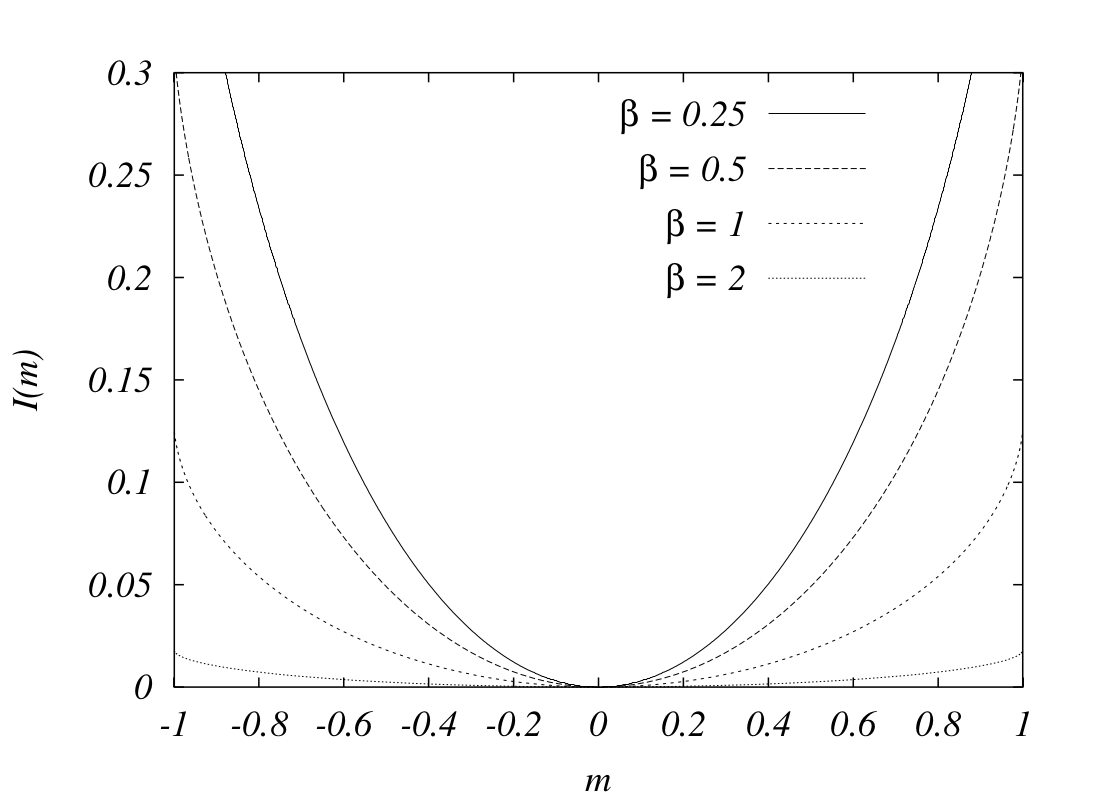
\includegraphics[width = 0.8\textwidth]{rate_fn.png}
    \caption{Rate function for the magnetization of the one-dimensional ising model}
\end{figure}
\begin{flushleft}
\textbf{Inference from figure 1: }As $\beta$ increases i.e as temperature decreases the probability of large fluctuations increases.
\end{flushleft}


\end{document}
